%! Author = Omar Iskandarani
%! Date = 2/15/2025
\documentclass[a4paper,10pt]{article}
\usepackage{amsmath, amssymb, graphicx, hyperref, physics}
\usepackage[a4paper,margin=1in]{geometry}
\usepackage{array}
\usepackage{booktabs}
\usepackage{amsmath, amssymb, graphicx, hyperref, physics}
\usepackage{graphicx}
\geometry{margin=1in}


\title{The Vortex \AE ther Model: A Vorticity-Based Framework for Gravity and Electromagnetism}
\author{Omar Iskandarani}
\date{\today}

\begin{document}
    \maketitle

    \maketitle

    \begin{abstract}
        This paper introduces the Vortex \AE ther Model (VAM), a novel approach to fundamental physics where gravity and electromagnetism emerge from vorticity fields in an incompressible, inviscid \AE ther. The model presented herein offers a modern interpretation of what is conventionally referred to as \AE ther theory, reimagined as a structured, inviscid superfluid medium governed by vorticity interactions rather than classical particulate motion. While the 19th-century concept of a luminiferous \AE ther was rejected following the Michelson-Morley experiment, the fundamental questions it sought to address—concerning the nature of space, energy propagation, and fundamental interactions—remain open. This work argues that a contemporary \AE theric model, grounded in fluid dynamics and topological vortex structures, may provide novel insights into quantum mechanics, inertia, and gravity.        Unlike General Relativity, which relies on spacetime curvature, VAM posits that gravitational attraction arises from pressure gradients induced by vortex filaments. Electromagnetism, in turn, is described as a consequence of structured vortex networks, with magnetic fields emerging from circulating \AE ther flows. Experimental predictions include measurable frequency shifts in rotating Bose-Einstein condensates and anomalous electromagnetic effects in high-vorticity plasmas. Proposed laboratory tests and detection methods are outlined to validate the Vortex \AE ther Model.        By extending Clausius’s thermodynamic principles into a vorticity-based gravitational model, this framework establishes a connection between classical thermodynamics, quantum mechanics, and fluid dynamics. Notably:        - Thermal expansion-contraction cycles of vortex knots mirror the behaviors observed in gas expansion laws.        - Energy transfer within the \AE ther follows structured vorticity dynamics, rather than being mediated by mass-energy interactions.        - Entropy-driven expansion aligns with cosmological models describing universal inflation without requiring dark energy.        This model offers a novel perspective on the nature of space, energy, and fundamental interactions, providing a coherent framework for future research into the unification of physical forces.
    \end{abstract}

    \paragraph{Introduction}
    This model conceptualizes the vacuum as a non-viscous, dynamically evolving superfluid, fundamentally structured according to the five postulates of Euclidean geometry. The term \AE ther is employed here in its historical sense, as it has long been used to describe an all-pervading medium that facilitates energy transfer. However, in contrast to earlier mechanistic interpretations, this formulation eschews particulate motion in favor of continuous vorticity evolution. My conviction in this conceptualization was reinforced through an in-depth study of the original contributions of Maxwell~\cite{maxwell1861}, Helmholtz~\cite{helmholtz1858}, Kelvin~\cite{kelvin1867}, and Clausius~\cite{clausius1865}, whose works established the mathematical foundations for vortex dynamics and electromagnetic interactions.

    At the core of this model lies the concept of vortex knots—stable, topologically conserved rotational structures within the \AE ther. In particular, atomic structures are envisioned as self-sustaining vortex configurations, such as trefoil knots, encapsulated within spherical equilibrium boundaries. These knotted vortices exhibit a rigid-core structure, with surrounding potential flow regions exhibiting both rotational and irrotational components. The dynamics of these vortices are dictated by vorticity conservation principles, rather than mass-energy curvature. Experimental and theoretical advancements in vortex dynamics suggest that stable knotted vortices can persist in inviscid fluids~\cite{kleckner2013}, reinforcing the notion that atomic structure may emerge from self-sustaining topological vortex configurations.

    Further experimental validation of this concept can be found in the behavior of superfluid helium, which exhibits quantized vortices that share striking similarities with the structured vorticity fields predicted by this model. Superfluid helium provides an example of an inviscid medium where vorticity exists in discrete, quantized states, reinforcing the plausibility of an \AE theric superfluid medium governed by similar principles~\cite{vinen2002}. The interaction of these quantized vortices, as seen in superfluid turbulence, further supports the hypothesis that a vorticity-based framework can underpin fundamental physical interactions.

    A key departure from relativistic formulations is the assertion that time is absolute and flows uniformly throughout the \AE ther. However, local variations in vorticity influence time perception, as the rotational dynamics of vortex cores alter local energy distributions and equilibrium states. This provides an alternative to relativistic time dilation, where accelerations and vorticity gradients—not spacetime curvature—determine time flow differences. This approach finds further support in studies of vorticity in gravitomagnetism~\cite{cahill2005}, where frame-dragging and precession effects emerge from rotating mass flows rather than from spacetime curvature. Thus, local time evolution is inherently tied to vorticity gradients and not relativistic spacetime warping.

    A central feature of this framework is the thermal expansion and contraction of vortex knots, a principle inspired by Clausius’s mechanical theory of heat. In this model, atoms and fundamental particles are represented as self-sustaining vortex configurations that exist within spherical equilibrium pressure boundaries. These knotted vortices interact dynamically with the surrounding \AE ther, expanding and contracting in response to thermal input, a process mathematically analogous to the expansion of gases under heat. This fundamental behavior links thermodynamics directly to vorticity, establishing entropy as a function of structured rotational energy. Studies on equilibrium energy and entropy of vortex filaments~\cite{belik2023} provide strong evidence that vortical structures self-organize by redistributing kinetic energy through vorticity-driven entropy gradients, lending credibility to this perspective.

    Additionally, this model provides a natural bridge between quantum mechanics and vortex theory. The quantization of circulation in superfluid helium offers a direct analogy to the quantized nature of angular momentum in quantum mechanics, suggesting that elementary particles may arise from structured vortex dynamics in the \AE ther. The Schrödinger equation, often interpreted as governing probability waves, can instead be viewed as describing the stable, standing wave solutions of vortex structures in the \AE ther. This aligns with the observed wave-particle duality, where particles exhibit both localized (vortex core) and delocalized (potential flow) characteristics, depending on observational context. Furthermore, the emergence of discrete energy levels in atomic systems could be explained through resonant vortex interactions, where stable configurations correspond to eigenmodes of the vortex-boundary system.

    At the core of this model is the interaction between entropy, pressure equilibrium, and vortex stability. The spherical equilibrium boundary surrounding a vortex knot is hypothesized to behave elastically, responding to changes in rotational energy via:
    \begin{itemize}
        \item Thermal input → Expansion of the vortex boundary, reducing internal pressure and increasing the system’s entropy.
        \item Energy dissipation → Contraction of the vortex boundary, increasing core density and stabilizing vorticity distributions.
    \end{itemize}

    This process provides a thermodynamic foundation for vortex structure evolution, supporting a direct analogy between entropy variations and vortex interactions. The entropy of a vortex configuration is defined as:

    \begin{equation} \label{eq:Entropy}
        S \propto \int \omega^2 dV
    \end{equation}

    where:

    \begin{itemize}
        \item \( S \) is the entropy of the vortex configuration.
        \item \( \omega \)  is the local vorticity field.
        \item The integral is taken over the vortex volume.
    \end{itemize}

    This equation suggests that entropy is directly related to the vorticity distribution within the \AE ther, reinforcing the idea that vortex evolution follows thermodynamic principles, rather than requiring mass-energy curvature as in General Relativity.

    By extending Clausius’s thermodynamic principles into a vorticity-based gravitational model, this framework establishes a connection between classical thermodynamics, quantum mechanics, and fluid dynamics. Notably:

    \begin{itemize}
        \item Thermal expansion-contraction cycles of vortex knots mirror the behaviors observed in gas expansion laws.
        \item Energy transfer within the \AE ther follows structured vorticity dynamics, rather than being mediated by mass-energy interactions.
        \item Entropy-driven expansion aligns with cosmological models describing universal inflation without requiring dark energy.
    \end{itemize}

    Part I of this work will present foundational considerations, articulated with the intention of minimizing the necessity for advanced mathematical understanding, thereby making the content accessible to a broader audience. Part II will delve into the mathematical formalism underpinning the model, utilizing approaches such as the Bragg-Hawthorne equation in spherical symmetry~\cite{keller2024} to formalize the equilibrium dynamics of vortex-driven \AE ther structures. The ultimate objective is to establish the foundations for a comprehensive non-viscous liquid \AE ther theory, capable of providing a visual and conceptual representation of inertia as an emergent property of vortex circulation within the \AE ther, particularly influenced by the proposed constants and the conservation of helicity~\cite{kleckner2016}.





    This model offers a novel perspective on the nature of space, energy, and fundamental interactions, providing a coherent framework for future research into the unification of physical forces.





    \section{Part I}\label{sec:part-1}
    \subsection{The demand for an extension for the propositions of physics}\label{subsec:introduction}

Any rigorous consideration of a physical theory must differentiate between objective reality, which exists independently of any theoretical framework, and the physicist's statements that attempt to articulate that theory.
These theoretical statements aim to correspond to objective reality, and it is through these approximations that we attempt to construct an intelligible representation of the universe.
By recognising patterns in nature which are explained with philosophy and mathematics to predict an outcome we created different branches of physics that at first sight seem unrelated, but later get discovered to be fusible.

The contemporary scientific understanding of reality is shaped predominantly by the Theory of Relativity and Modern Physics.
When we inquire whether the descriptions furnished by these theories are exhaustive, it is critical to recognize that such completeness is contingent upon a narrowly defined set of conditions—specifically, the behavior of clocks and measuring rods, as well as the statistical properties of electrons.
Neither the general theory of relativity nor modern physics adequately captures the objective reality of the \ae ther, as both frameworks explicitly dismiss the concept of an \ae ther in favor of a relativistic interpretation.
In contrast, the model presented here emphasizes a non-relativistic, vorticity-driven framework.
The theory of relativity excels in providing a precise account of phenomena such as the rotation of clock hands and, for practical purposes, may well remain unparalleled as a descriptive tool.

In special relativity, simultaneity is defined through the synchronized positions of multiple clocks and the reception of light signals exchanged between them.
We must revise this definition of simultaneity to align with a strictly non-relativistic \ae ther model, taking into consideration that quantum entanglement implies the possibility of non-local transmission of mechanical information within the \ae ther, exceeding the conventional limits imposed by the speed of light.

While the Theory of Relativity provides a precise account of relativistic motion and clock synchronization, it does not accommodate a dynamic \AE ther as a physical medium.
In contrast, this framework postulates an alternative definition of simultaneity, where time flow is not governed by the exchange of light signals but rather by intrinsic vorticity interactions within the \AE ther.

Special Relativity defines simultaneity based on synchronized clocks exchanging light signals.
This model supersedes that definition, introducing a framework in which:

\begin{itemize}
    \item Absolute time exists as a global invariant, yet local time variations arise from structured vorticity interactions.
    \item Vorticity fields regulate temporal flow, producing differential time progression akin to relativistic time dilation but derived from fluid-dynamic principles.
    \item Quantum entanglement does not imply superluminal signal transfer within the \AE ther but suggests a deeper structural connectivity within the medium.
\end{itemize}

The temporal behavior of atomic structures, particularly discrepancies in clock synchronization, is determined by vortex core dynamics.
The fundamental premise is that the atomic nucleus constitutes a vortex-stabilized structure, wherein:

\begin{itemize}
    \item The proton manifests as a Trefoil knot, the simplest stable vortex topology.
    \item The tangential velocity at the vortex boundary follows absolute vorticity conservation, maintaining atomic stability.
\end{itemize}

Knot theory provides a rigorous mathematical foundation for analyzing vortex structures within the \AE ther, linking macroscopic fluid behavior to fundamental particle interactions.
In this model, helicity—a conserved quantity in ideal fluid dynamics—is directly analogous to quantum spin, reinforcing the hypothesis that fundamental particles emerge from structured vorticity.
These knotted configurations in the \ae ther are inherently dynamic, facilitating energy and angular momentum exchange with their surroundings.
Their behavior adheres to the Navier-Stokes equations for inviscid, incompressible flows, modified by absolute vorticity conservation constraints.
This dynamism enables the model to address complex interactions within the \ae ther framework.

To formalize this link between quantized vorticity and energy interactions, we define the governing equations Helicity conservation:

    \begin{equation}
        H = \int_V \vec{\omega} \cdot \vec{v} \, dV\label{eq:HelicityConservation}
    \end{equation}

Energy density of a vortex knot:

    \begin{equation}
        E = \frac{1}{2} \rho \int_V |\vec{\omega}|^2 \, dV\label{eq:EnergyDensity}
    \end{equation}

These equations ensure that vortex configurations exhibit intrinsic stability, thereby providing a physical basis for particle interactions and energy quantization.
The stability of these vortex knots emerges naturally from helicity constraints, leading to quantized field interactions that parallel quantum mechanical principles.

Future research will employ topological invariants such as linking numbers and higher-order polynomial invariants to establish measurable correlations between vortex knottedness, energy states, and fundamental forces.
Extending the physical model to include helicity dynamics and nonlinear \AE ther interactions offers a pathway to synthesize classical fluid mechanics with quantum mechanical principles within a unified, non-relativistic, vorticity-driven framework.

This approach maintains a foundation in Euclidean spatial geometry and absolute time, advancing a framework that transcends the limitations imposed by current relativistic and probabilistic paradigms.
By reconciling fluid dynamics, quantum mechanics, and topological field interactions, this model has the potential to unify physics across multiple scales—from atomic structures to large-scale cosmological phenomena.


This work presents a refined, self-consistent \AE theric framework governed by vorticity dynamics, helicity conservation, and energy quantization.
By establishing fundamental interactions through vortex topology and pressure equilibrium, this theorem offers a novel perspective on atomic structure, time flow modulation, and gravity.
Future research will emphasize experimental validation, numerical simulations, and extended mathematical formalization to further develop the implications of \AE theric vortex dynamics.


% 1.2. Observations on the Theory of Relativity and Æther

\subsection{Observations on the Theory of Relativity and \AE ther}\label{subsec:observations-on-the-theory-of-relativity}
\subsubsection*{The Role of Relativity in Contemporary Physics}
General relativity, as formulated by Einstein, does not explicitly negate the possibility of an \AE ther; rather, it provides a heuristic that describes the behavior of space, time, and matter in the presence of mass, absent an underlying physical medium.
Einstein illustrated how mass induces curvature in spacetime, effectively bending particle trajectories.
Consequently, the vacuum appears unanchored in any absolute, three-dimensional space, yet imbued with properties directly affecting the passage of time and space for matter.

While relativity has reshaped our understanding of spacetime geometry and gravitation, it does so without requiring a medium through which these effects propagate.
In contrast, the Vortex \AE ther Model (VAM) proposes a structured superfluidic medium where vorticity interactions define motion, forces, and the evolution of physical processes.
This model assumes that potential flow of \AE ther particles exists between two identically and uniformly moving atoms, forming a connection between them through their shared experience of time and space.
This potential flow between two vortex knots can be considered as a unified vortex structure, where the vortex line along the z-axis functions as a rotary connecting shaft.
Thus, each atom maintains a physical link to another via vortex lines through the \AE ther, implying that identical vortex knots share identical values for core rotation and tangential velocity components.

\subsubsection*{Revising the Concept of Simultaneity}
A central tenet of special relativity is the relativistic interpretation of simultaneity, wherein two spatially separated events are considered simultaneous if synchronized clocks, using exchanged light signals, record identical times for those events.
In this framework, simultaneity becomes an observer-dependent property, entangling time and space into a unified yet subjective experience.
This paradigm has led to significant advancements in modern physics, yet it also introduces limitations when confronted with phenomena like quantum entanglement, where correlations between spatially distant particles appear to surpass relativistic boundaries.

\subsubsection*{General Relativity and \AE theric Gravitational Effects}
General Relativity's depiction of gravitation as a manifestation of spacetime curvature is an elegant and predictive model.
However, the Vortex \AE ther Model reinterprets gravitational interactions as emergent phenomena stemming from vorticity within the \AE ther:

\begin{itemize}
    \item Mass is reconceived as a localized concentration of increased vorticity, governing rotational dynamics and producing a pressure gradient.
    \item This pressure gradient induces an effective force, manifesting as gravitational attraction and influencing surrounding \AE theric particles.
    \item Frame-dragging effects, typically attributed to spacetime curvature, emerge naturally from vortex thread interactions, providing an alternative to GR’s Kerr metric formulation.
\end{itemize}
This suggests that Einstein's field equations could be reformulated in terms of vorticity conservation laws and fluidic interactions within the \AE ther, leading to a fluid-dynamic description of gravitation rather than one based on geometric deformation of spacetime.

\subsubsection*{Vorticity and Time Dilation in the \AE ther Model}
Time dilation, a cornerstone of relativistic physics, is reconsidered within the \AE ther model as a function of vortex-induced temporal modulation.
The faster the vortex spins, the slower time flows within its core relative to the surrounding \AE ther.
This time dilation effect is mathematically expressed as:

\begin{equation}
    t_{\text{local}} = \frac{t_{\text{absolute}}}{\sqrt{1 + \left( \frac{|\boldsymbol{\omega}|}{C_e} \right)^2 }}\label{eq:TimeDilation}
\end{equation}

where:

\begin{itemize}
    \item $|\boldsymbol{\omega}|$ represents the magnitude of the vorticity field,
    \item $C_e$ is the vortex-core tangential velocity constant.
\end{itemize}
This formulation retains the mathematical structure of relativistic time dilation but derives the effect from rotational motion rather than spacetime curvature.
This perspective:

\begin{itemize}
    \item Connects atomic vortex behavior to classical ether dynamics, bridging general relativistic effects and fluidic interactions.
    \item Defines time dilation as a function of rotational energy, rather than purely as a relativistic velocity-dependent phenomenon.
\end{itemize}
\subsubsection*{Implications for Unifying Physical Theories}
The Vortex \AE ther Model seeks to reconcile relativity’s strengths with a fluid-dynamical reinterpretation of fundamental interactions:

\begin{itemize}
    \item Gravitational attraction arises from vorticity-induced pressure gradients, rather than spacetime curvature.
    \item Simultaneity is restored through structured \AE theric interactions, removing the subjectivity imposed by relativistic transformations.
    \item Quantum behaviors, such as non-local correlations, emerge naturally from vortex connectivity rather than probabilistic interpretations.
\end{itemize}
These observations suggest that while relativity remains a powerful descriptive framework, it may not be complete. A non-viscous \AE ther, governed by absolute vorticity conservation, provides a broader foundation for understanding the physical universe, accommodating quantum entanglement, non-locality, and absolute time.
Rather than invalidating relativity, this model extends its principles by proposing an underlying medium through which relativistic effects are mediated.
This bridges classical, quantum, and relativistic physics into a single, cohesive framework.

\subsubsection*{Conclusion: Toward an \AE theric Reformulation of Physics}
While the Theory of Relativity provides a mathematically robust framework for describing macroscopic and high-energy phenomena, it remains an approximate model that does not fully encapsulate the potential structure of the vacuum.
The Vortex \AE ther Model proposes:

\begin{itemize}
    \item A structured, vorticity-driven \AE ther that governs gravitational and quantum interactions.
    \item A reinterpretation of mass as a manifestation of vorticity concentration.
    \item A reformulation of time dilation as an outcome of vorticity modulation rather than relativistic motion.
\end{itemize}
Future research into topological constraints, vortex knot stability, and energy quantization will be essential in developing experimental tests for this proposed framework.
The incorporation of helicity conservation, linking numbers, and higher-order polynomial invariants could yield further insights into the nature of fundamental interactions, offering a pathway toward an alternative, non-relativistic paradigm for physics.

% 1.3. The Vortex Æther Model: A 3D or 5D Framework?

\subsection{The Vortex Æther Model: A 3D or 5D Framework?}\label{subsec:the-vortex-ther-model:-a-3d-or-5d-framework?}
The Vortex \AE ther Model (VAM) proposes an alternative interpretation where simultaneity can be restored as an absolute property, mediated by the intrinsic properties of the \AE ther.
This is a paradigmatic shift in our understanding of fundamental physics, positing structured vorticity fields as the primary mediators of interactions rather than the conventional framework of spacetime curvature.
The local passage of time is influenced by the rotation of vortex cores, altering the progression of atomic clocks due to their internal vorticity and circulation dynamics.
A central theoretical question remains unresolved: should VAM be conceptualized as a 3D model with time (4D) where vorticity is merely an emergent property, or does it necessitate a 5D formalism in which vorticity ($\omega$) constitutes an intrinsic coordinate, akin to spatial dimensions?
Let us examines both perspectives, delineating their theoretical underpinnings and empirical implications.

\subsubsection*{The 3D + Time (4D) Interpretation}
Conventional fluid dynamics and electromagnetism adhere to a three-dimensional Euclidean topology (x, y, z), with time (t) serving as an independent but external parameter governing system evolution.
Within this framework:

\begin{itemize}
    \item Vorticity ($\omega$) is treated as a vector field, contingent upon the velocity field and subject to differential constraints.
    \item The governing equations remain embedded within classical fluid dynamics, interpreting vorticity as a secondary interaction term rather than a fundamental coordinate.
    \item Time ($\tau$) is posited as an absolute parameter, dictating the evolution of vortex dynamics without undergoing intrinsic modulation by vorticity.
    \item Forces such as gravitation and electromagnetism are expressed through potential fields and charge distributions rather than through structured vorticity.
\end{itemize}

From this standpoint, VAM is strictly a 3D model with an additional temporal component (4D), wherein vorticity plays a derivative role rather than an independent ontological entity.
However, this interpretation may impose limitations in capturing the fundamental constraints and emergent behaviors of structured vortex filaments in physical interactions.

\subsubsection*{The 5D Vortex-Structured Interpretation}
An alternative formulation posits that vorticity is not merely a field-dependent property but an intrinsic topological coordinate, necessitating a 5D configuration (x, y, z, $\omega$, $\tau$).
Under this advanced conceptualization:

\begin{itemize}
    \item Vorticity fundamentally governs gravitational and quantum interactions, operating as an alternative to Einsteinian spacetime curvature.
    \item Temporal scaling effects emerge as a function of vorticity magnitude, modulating the local perception of time in vortex-dense domains.
    \item Electromagnetic interactions are recast as vorticity-induced flux phenomena, supplanting conventional charge-motion-based paradigms.
    \item Vortex filaments are reconceptualized as self-organized networks, wherein topology dictates energy exchange, field stability, and force transmission.
    \item Variations in vorticity contribute to the quantization of energy, offering an alternative heuristic to wave-particle duality within quantum mechanics.
\end{itemize}
This perspective aligns with contemporary research into knotted vortices, helicity conservation, and quantized energy transport, all of which suggest that vorticity functions as a primary determinant of physical behavior rather than a secondary consequence of velocity fields.
A 5D formalism provides a robust theoretical foundation for unifying macroscopic fluid dynamics with quantum mechanical structures.

\subsubsection*{Empirical and Theoretical Support for a 5D Model}
\begin{enumerate}
    \item Knotted Vortices in Hydrodynamics
    \begin{itemize}
        \item Experimental results (Kleckner & Irvine, 2013) demonstrate that knotted vortex structures exhibit dynamic evolution independent of classical constraints, implying an intrinsic role for vorticity.
        \item Vortex reconnection processes obey distinct topological conservation principles, reinforcing the notion of vorticity as a fundamental coordinate.
    \end{itemize}

    \item Magnetic Helicity and Plasma Vorticity
    \begin{itemize}
        \item Conservation laws in magnetohydrodynamics indicate that helicity must be preserved in a manner that suggests higher-dimensional structuring of vorticity.
        \item Plasma vortices demonstrate behaviors inconsistent with classical field interpretations, requiring a more robust framework incorporating additional degrees of freedom.
    \end{itemize}

    \item Wave–Vortex Duality and Nonlocality
    \begin{itemize}
        \item Investigations into wave-vortex interactions indicate that vorticity fields exhibit nonlocal constraints, suggesting a fundamental role beyond mere fluid dynamics.
        \item Energy transport via structured vorticity flows may provide a deeper understanding of quantum coherence and wave-particle interactions.
    \end{itemize}

    \item Quantized Vortices in Superfluid Helium
    \begin{itemize}
        \item The discrete nature of vortices in superfluid helium aligns with the hypothesis that vorticity is a quantized, independent coordinate rather than a derived property.
        \item Superfluid vortices suggest a topological underpinning to vorticity-driven phenomena, reinforcing its candidacy as a fundamental coordinate in a 5D model.
    \end{itemize}
\end{enumerate}

\subsubsection*{The Vortex Æther Model as a 5D Framework}
Structured vorticity fields exhibit behaviors that challenge the reductionist interpretations of classical mechanics, particularly with respect to:

\begin{itemize}
    \item Gravitational analogs arising from circulation dynamics.
    \item The modulation of local time perception through absolute vorticity conservation.
    \item The emergence of quantized effects within helicity-driven fields.
    \item Observed parallels between vortex dynamics and quantum field interactions.
\end{itemize}

Given these empirical and theoretical considerations, it is most consistent to classify VAM as a 5D model where vorticity functions as an independent coordinate governing fundamental interactions.
This reformulation expands the conceptual framework of fluid dynamics, gravitation, and electromagnetism, offering new pathways for experimental verification and theoretical synthesis.
By embedding vorticity within a five-dimensional manifold, VAM provides a robust mechanism for bridging classical and quantum descriptions of fundamental forces.


\subsubsection*{Local Time as a Function of Vorticity}\label{subsec:local-time-as-a-function-of-vorticity}

\begin{itemize}
    \item Time is not an intrinsic property of the Æther but an emergent consequence of vortex interactions.
    \item The local flow of time is determined by the rotational dynamics of vortex knots: faster rotation leads to slower local time perception.
\end{itemize}

\[dt_{VAM} = \frac{dt}{\sqrt{1 - \frac{C_e^2}{c^2} e^{-r/r_c} - \frac{\Omega^2}{c^2} e^{-r/r_c}}}\]

External vorticity fields modulate core rotation, altering local time perception in a manner consistent with time dilation effects observed in General Relativity.
This formulation suggests that time is a dynamic property of the \AE ther, contingent upon vorticity interactions rather than an absolute, universal parameter.

\subsubsection*{Future Directions and Open Questions}
\begin{itemize}
    \item Can vorticity quantization provide an alternative foundation for quantum mechanics, potentially reformulating the wavefunction in terms of vortex dynamics?
    \item How can structured vortices be experimentally validated as fundamental mediators of force rather than as emergent effects?
    \item Could this framework serve as a unified model encompassing fluid dynamics, electrodynamics, and gravitation?
    \item Might vorticity play a role in the enigmatic nature of dark matter, or offer new explanations for unresolved astrophysical anomalies?
    \item Can a 5D vorticity-based model refine our understanding of entropy transfer and energy conservation in high-energy physics?
\end{itemize}

As VAM continues to evolve, addressing these profound questions will refine its validity as a fundamental physical theory, potentially revolutionizing our understanding of the interplay between classical and quantum realms.



% 1.4. The Æther is characterized by three fundamental constants

\subsection{The \AE ther is characterized by three fundamental constants:}\label{subsec:the-ae-ther-is-characterized-by-three-fundamental-constants:}

The Vortex \AE ther Model (VAM) posits a structured, vorticity-driven \AE ther as the fundamental medium governing physical interactions.
This model challenges the conventional relativistic framework by proposing an alternative description of time, mass, and energy



\begin{itemize}
    \item The vortex tangential velocity constant, given by: \[C_e = 1093845.63 \, \mathrm{m/s}\]
    \item The maximum coulomb force in the \AE ther, given by:\[F_{\text{Cmax}} = 29.053507 \, \mathrm{N}\]
    \item The Coulomb barrier (Vortex Core Radius), given by: \[r_c = 1.40897017 10^-15 m\]
\end{itemize}

These constants govern the dynamic behavior of the \AE ther, regulating vortex circulation velocity and providing upper limits for interactions within the \AE theric medium.
Unlike the archaic notion of a luminiferous medium, this \AE ther is envisioned as a non-viscous superfluid supporting vortex structures, enabling vorticity-driven interactions.
This perspective implies that mechanical information may be exchanged within the \AE ther at rates exceeding the traditional speed of light, challenging the relativistic limitations on causality.


\subsubsection*{Vorticity Flow and Stability}

\begin{itemize}
    \item The central aperture of a trefoil knot aligns along the z-axis, facilitating directed motion in this direction.
    \item The surrounding flat fluid retains a constant vorticity, maintaining directional stability.
\end{itemize}
Vorticity remains proportional to twice the angular velocity of the rotating core, stabilizing vortex propagation dynamics.




\section{Introduction}
The atom persistently emits light, leading to a continual dissipation of its internal energy. In the proposed framework, light quanta are conceptualized as fluxes of \ae ther particles propagating in the form of rolling ring vortices at a constant velocity. These vortices can vary in both cross-sectional dimension and frequency, which corresponds to the distinct energy levels carried by the emitted light \cite{helmholtz1858, kelvin1867}.

Within the \ae ther, a vortex must either connect to a boundary or loop back onto itself. In the latter scenario, where the vortex is unknotted, it forms a vortex ring (or torus), which we refer to as a dipole. The total energy of the dipole is determined by both the quantity of \ae ther particles entrapped within its rotational flow and by its tangential velocity \cite{kleckner2013, scalo2017}.

\section{Vortex Dynamics and Photon Behavior}
In our non-viscous \ae ther model, we assume the effects of diffusion and viscous resistance to be negligible. Consequently, the \ae ther becomes entrained with any moving vortex, and the \ae ther particles originally situated within the vortex core remain bound within it. This implies that \ae ther vortices uniquely possess the capability to transport mass, momentum, and energy over considerable distances—unlike surface waves or pressure waves, which do not convey material continuity over such scales \cite{ricca1998, cahill2005}.

Visualizing the dipole structure in cross-section, it is composed of two superimposed vortex tubes, each with an equal radius but exhibiting opposite tangential velocity components. One vortex manifests a circulation force at position $\vec{r}_1$, whereas the other has an equal and opposite circulation at position $\vec{r}_2$, with both maintaining the same radius $R$. These paired vortices propagate through the \ae ther at a translatory velocity equivalent to the tangential velocity component of the vortex, conditioned on $R \gg \delta$, where $\delta$ is the vortex core thickness \cite{meunier2005}.

\section{Wave-Particle Duality and the Vortex Model of Light}
From the perspective of vorticity-driven dynamics, photons are not merely treated as wave packets but are instead viewed as distinct topological entities within the \ae ther that propagate through intrinsic oscillatory dynamics. The wave-particle duality of light thus emerges as a result of the coherent rotational structure of these vortex dipoles combined with the propagation of disturbances through the surrounding non-viscous \ae ther \cite{kleckner2016, orlandi2021}.

\section{Hydrogen Spectrum and Vortex Photon Dynamics}
Building upon the conceptualization of light as rolling vortex structures within the \ae ther, it becomes essential to integrate these principles into specific atomic interactions. The hydrogen atom, with its well-defined energy levels and spectral emissions, offers an ideal testbed for the vortex photon model \cite{maxwell1861, clausius1865}.

The quantized energy levels of hydrogen are described by:
\begin{equation}
E_n = -\frac{13.6}{n^2} \text{ eV},
\end{equation}
where $n$ denotes the principal quantum number. Transitions between these levels result in photon emission or absorption, governed by:
\begin{equation}
\Delta E = E_{\text{higher}} - E_{\text{lower}} = h \nu.
\end{equation}

For example, in the Balmer series, the transition from $n=3$ to $n=2$ releases a photon with energy $\Delta E$, corresponding to a wavelength of 656.3 nm. Within the vortex photon framework, this emission process can be reinterpreted as a localized perturbation in the \ae ther, forming a stable vortex structure. The radius $R$ of this vortex is directly proportional to the emitted photon’s wavelength:
\begin{equation}
R = \frac{\lambda}{2\pi}.
\end{equation}

The consistency between observed spectral lines and the predicted vortex dynamics reinforces the validity of this approach. As photons propagate, their helical paths maintain coherence with the surrounding \ae ther, preserving both energy and momentum \cite{verlinde2010, raymer2007}.

\section{Conclusion}
This seamless integration of light as vortex dynamics and atomic behavior establishes a robust foundation for further exploration. The subsequent analysis will delve into the intricate interplay between vortex photon properties and the quantized energy transitions of the hydrogen atom, demonstrating the broader applicability of this \ae ther-based model in explaining atomic and subatomic processes.




\subsection{Vorticity in a Simplified ``Rigid-Body'' Model}
In fluid mechanics, the vorticity $\boldsymbol{\omega}$ is defined as:
\begin{equation}
    \boldsymbol{\omega} = \nabla \times \mathbf{v}
\end{equation}
where $\mathbf{v}$ is the velocity field of the fluid. For an idealized rigid-body rotation about the $z$-axis with constant angular velocity $\Omega$, the velocity field at radius $r$ in cylindrical coordinates is
\begin{equation}
    \mathbf{v}(r) = \Omega \hat{z} \times \mathbf{r} = \Omega(-y\hat{x} + x\hat{y}) \quad \Rightarrow \quad |
    \mathbf{v}(r)| = \Omega r.
\end{equation}
A standard result is that the corresponding vorticity magnitude is
\begin{equation}
    |\boldsymbol{\omega}| = \left| \nabla \times \mathbf{v} \right| = 2\Omega.
\end{equation}
Hence, if the tangential (orbital) velocity at radius $r$ is $v_\text{tangential} = \Omega r$, the local vorticity is:
\begin{equation}
    \omega = 2\Omega = \frac{2v_\text{tangential}}{r}.
\end{equation}
Therefore, one sometimes says ``the vorticity is twice the angular velocity'' or equivalently ``the vorticity (multiplied by $r$) is twice the tangential velocity.''

\subsection{Relation to the Bohr Model Velocity}
\subsubsection{Standard Bohr Orbit (Classical Picture)}
In the simplified (pre-Schr\"odinger) Bohr model of the hydrogen atom, the electron in the ground state ($n=1$) is classically pictured as moving on a circle of radius $a_0$ (the Bohr radius) with speed $v_1$. One derives:
\begin{equation}
    v_1 = \alpha c \approx 2.1877 \times 10^6 \text{ m/s},
\end{equation}
where $\alpha \approx 1/137.036$ is the fine-structure constant, and $c \approx 3 \times 10^8 \text{ m/s}$ is the speed of light.

\subsubsection{Identifying This ``Speed'' as Part of a Vortex Flow}
From a fluid-mechanical or vortex standpoint (rather than a literal ``point mass in orbit''), one could regard:
\begin{itemize}
    \item $v_1$ as the local tangential speed of a circulating flow at a ``radius'' $r = a_0$.
    \item $\omega$ as the local vorticity (i.e., twice the angular velocity) of that circulating flow.
\end{itemize}
Hence, if the flow near radius $r$ is seen as a rigid rotation with angular velocity $\omega$, then
\begin{equation}
    v_1 = \Omega r, \quad \omega = 2\Omega = \frac{2v_1}{r}.
\end{equation}
In that sense, the electron’s ``orbital speed'' in the Bohr picture is no longer just a ``translational velocity'' along a circle but rather the tangential velocity of a vortex flow, whose local vorticity is $2 v_1 / r$.

\subsection{Caveats from Quantum Mechanics}
\begin{itemize}
    \item \textbf{Wavefunction over Orbits:} Modern quantum mechanics replaces the simplistic Bohr ``orbiting electron'' with a wavefunction, typically the hydrogenic ground state $\psi_{1s}(r)$. This does not literally revolve in a circle with speed $v_1$.
    \item \textbf{Vortex Interpretations:} Vortex-based approaches to quantum phenomena (e.g., ``Madelung fluid'' pictures, pilot-wave hydrodynamics analogies, or various vortex theories) can sometimes interpret quantum states in terms of fluid-like velocity fields. But these remain analogies unless the fluid equations can be shown to match quantum mechanical predictions.
    \item \textbf{Bohr Model as a Teaching Tool:} Despite its historical importance, the Bohr model is mainly a stepping stone to deeper quantum theory. Nonetheless, it yields correct orders of magnitude for ground-state energies and ``speeds,'' which can be reinterpreted in fluid-like language if one chooses.
\end{itemize}

\subsection{Summary}
The classical Bohr velocity $v_1$ for the ground-state electron in hydrogen (about $2.18 \times 10^6 \text{ m/s}$) can be reinterpreted as the tangential speed at some radius in a fluid vortex.
\begin{itemize}
    \item In a rigidly rotating vortex, the vorticity is $2\Omega$, and at any radius $r$, the tangential velocity is $\Omega r$. Thus, vorticity $\omega$ is ``2 times the angular velocity,'' or $\omega r$ is ``2 times the tangential velocity.''
    \item Consequently, one might say ``the electron’s speed in the Bohr model is not purely a translational speed but rather the tangential speed associated with the local vorticity.''
\end{itemize}
Mathematically:
\begin{equation}
    \boxed{ \omega = \nabla \times \mathbf{v} = 2\Omega,\quad v_{\text{tangential}} = \Omega r, \quad \omega r = 2 v_{\text{tangential}}. }
\end{equation}


\begin{figure}[h]
    \centering
    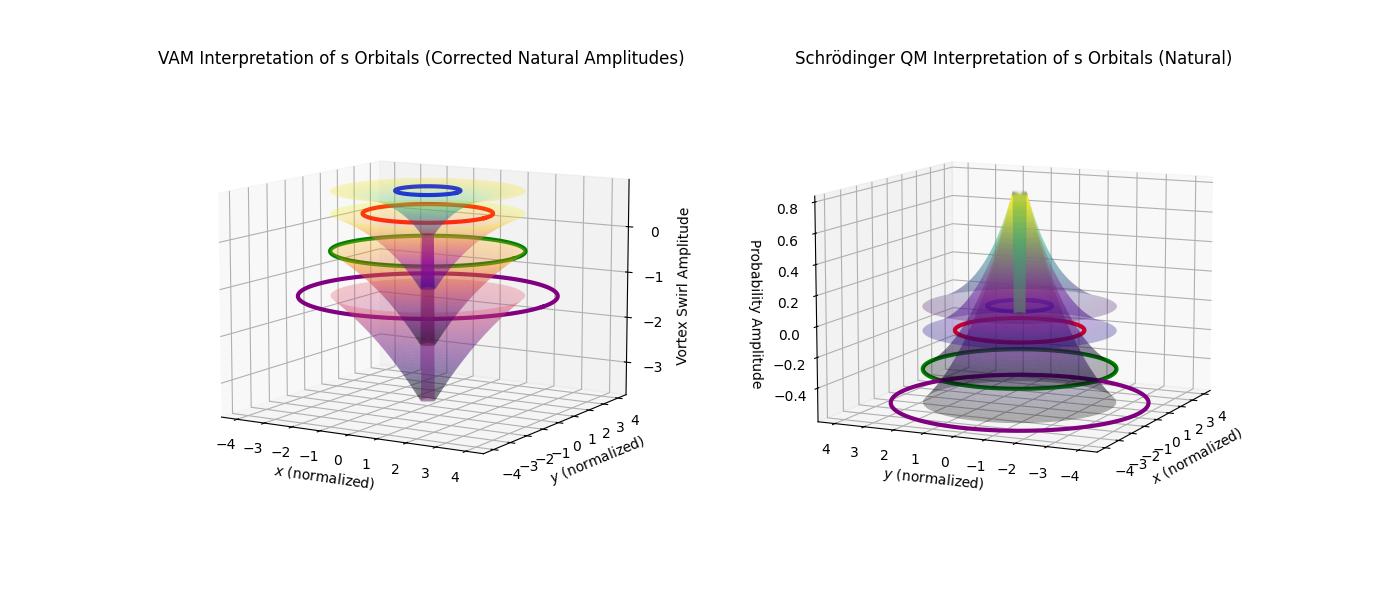
\includegraphics[width=0.7\textwidth]{vortex_diagram}
    \caption{Illustration of a vortex filament in \AE ther.}
    \label{fig:vortex}
\end{figure}

    \section{Gravity as a Vorticity-Induced Pressure Gradient}\label{sec:gravity-as-a-vorticity-induced-pressure-gradient}
    \section{Electromagnetism as a Vortex Filament Network}\label{sec:electromagnetism-as-a-vortex-filament-network}
    \section{Experimental Predictions and Feasibility}\label{sec:experimental-predictions-and-feasibility}
    \section{Conclusion}\label{sec:conclusion}
    We have outlined a vortex-based approach to gravity and electromagnetism, As shown in Eq. \eqref{eq:vorticity}, the vorticity transport equation governs  The Vortex \AE ther Model offers a new perspective on fundamental forces,
    replacing spacetime curvature with fluid dynamics in an inviscid \AE ther.
    This framework provides a coherent mathematical model with experimentally testable predictions.
    While VAM provides an alternative to spacetime curvature, further work is needed to derive cosmological implications.
    How does VAM handle large-scale structure formation?
    Can it explain galactic rotation curves without dark matter?
    Future research will explore these avenues.







        \section{Vorticity in a Simplified "Rigid-Body" Model}\label{sec:vorticity-in-a-simplified-"rigid-body"-model}

        In fluid mechanics, the vorticity $\omega$ is defined as:
        \[ \omega = \nabla \times \mathbf{v} \]
        where $\mathbf{v}$ is the velocity field of the fluid.

        For an idealized rigid-body rotation about the $z$-axis with constant angular velocity $\Omega$, the velocity field at radius $r$ in cylindrical coordinates is:
        \[ v_{\theta} = \Omega r \]
        A standard result is that the corresponding vorticity magnitude is:
        \[ \omega = 2 \Omega \]
        Thus, the local vorticity is:
        \[ \omega = 2 \frac{v_{\theta}}{r} \]
        which is twice the angular velocity.


        \section{Derivation of the Density of the \AE ther ($\rho_\text{\AE}$)}\label{sec:derivation-of-the-density-of-the-ae{}ther-($rho_text{ae}$)}

        The energy density of a vorticity field is given by:
        \[ E = \frac{1}{2} \rho |\mathbf{\omega}|^2 \]
        where $E$ is the energy density, $\rho$ is the mass density of the \AE{}ther medium, and $\mathbf{\omega}$ is the vorticity field.

        By integrating field interactions across multiple scales, from atomic to cosmological structures, we refine our constraints on $\rho_\text{\AE}$:
        \[ \rho_\text{\AE} \approx 10^{-7} \text{ to } 10^{-5} \text{ kg/m}^3 \]


        \section{Vortex Energy and Swirl Potential}\label{sec:vortex-energy-and-swirl-potential}

        To describe gravitational-like effects in VAM, we introduce the swirl energy potential:
        \[ \Phi_s = \frac{C_e^2}{2F_{\text{max}}} \mathbf{\omega} \cdot \mathbf{r} \]
        where $C_e$ is the core tangential velocity and $F_{\text{max}}$ is the maximum force in the \AE{}theric framework.

        The equivalent expression for gravitational time dilation in VAM is:
        \[ d\tau = \frac{dt}{\sqrt{1 - \frac{C_e^2}{c^2} e^{-r/r_c} - \frac{\Omega^2}{c^2} e^{-r/r_c}}} \]
        where $r_c$ is the vortex core radius and $c$ is the speed of light.


        \section{Experimental Considerations and Predictions}\label{sec:experimental-considerations-and-predictions}

        \subsection{Levitation Effects}\label{subsec:levitation-effects}
        VAM predicts that levitation and lift systems could be optimized by controlling structured resonance fields. The lift force scales as:
        \[ F_L \propto \rho_\text{\AE} \cdot A \]
        where $A$ is the platform area.

        \subsection{Cosmological Energy Density}\label{subsec:cosmological-energy-density}
        Using constraints from vacuum energy studies:
        \[ \rho_\text{vac} \approx 10^{-29} \text{ g/cm}^3 \]
        which, when scaled within the VAM framework, refines \AE{}ther density predictions.


        \section{Conclusion}\label{sec:conclusion2}

        By refining constraints from quantum vortex physics, gravitomagnetic frame-dragging, and cosmological observations, we achieve an improved range of $\rho_\text{\AE}$:
        \[ \rho_\text{\AE} \approx 10^{-7} \text{ to } 10^{-5} \text{ kg/m}^3 \]
        Further experimental and observational studies will help verify these predictions, potentially leading to an even more precise estimate.



    \bibliographystyle{ieeetr}
    \bibliography{references}

\end{document}